\documentclass[TS,lsstdraft,authoryear,toc]{lsstdoc}
\input{meta}

% Package imports go here.

% Local commands go here.

%If you want glossaries
%\input{aglossary.tex}
%\makeglossaries

\title{The effect of louvers on delivered image quality}

% This can write metadata into the PDF.
% Update keywords and author information as necessary.
\hypersetup{
    pdftitle={The effect of louvers on delivered image quality},
    pdfauthor={Elana K.Urbach},
    pdfkeywords={}
}

% Optional subtitle
% \setDocSubtitle{A subtitle}

\input{authors}

\setDocRef{TSTN-064}
\setDocUpstreamLocation{\url{https://github.com/lsst-tstn/tstn-064}}

\date{\vcsDate}

% Optional: name of the document's curator
% \setDocCurator{The Curator of this Document}

\setDocAbstract{%
We have gone from zero working louvers at LSSTCam's first light to twelve working louvers one year later. We present results on the effect of these louvers on image quality in a progressive manner and we give upper and lower value estimates on how much additional louvers would improve seeing at the Simonyi Telescope.
}

% Change history defined here.
% Order: oldest first.
% Fields: VERSION, DATE, DESCRIPTION, OWNER NAME.
% See LPM-51 for version number policy.
\setDocChangeRecord{%
  \addtohist{1}{2026-07-06}{Unreleased.}{Urbach}
}


\begin{document}

% Create the title page.
\maketitle
% Frequently for a technote we do not want a title page  uncomment this to remove the title page and changelog.
% use \mkshorttitle to remove the extra pages
\section{Introduction}
Since early commissioning we have been incorporating different dome components to our venting strategy to improve image quality. A first stage had the dome airflow at night dominated by air coming through the dome shutter, a second stage added the incremental operation of six electro-mechanical louvers and a third stage incorporated at once six additional pneumatic louvers.  Having these different stages we were able to quantify the per-louver image quality improvement linked with louver ventilation, separated from seasonal and environmental relations.

\section{Data}
We consider the time period July 1 2025 to June 14 2026 in our analysis. This dataset includes a time period with no louvers (from July 1 2025), the ramp up of electro-mechanical louvers (Oct 20 - Nov 28 2025), the steady six electro-mechanical louver operation stage (Nov 29 2025 - April 22 2026) and the period when we additionally operated the pneumatic louvers (from April 23 2026 to June 15 2026). Our image quality metric is the calculated donut\_blur\_FWHM in arcsec units ($IQ_{db}$ hereafter) on non-y band FBS images. A louver is considered open when it has $>$90\% aperture using EFD telemetry during the six louver (B1, E1, E2, H1, H2, M1) stage. The pneumatic louvers (A1, C1, D1, I1, L1, N1) lack telemetry information and are assumed to be always open while on-sky, their count is added as a fixed number (6) after April 23 2026. Our working variable is $D(n)$, the step function that traces the number of operational louvers on a given night. Additionally, we considered as covariates the external wind speed, the in-dome/outside temperature differential, effective dome airspeed, wind direction regime, TMA elevation, relative humidity, and outside temperature.                                          

\section{Methods}
Our main goal is to isolate the impact of the louvers in our image quality metric, for this we were focused on two main methods. An Interrupted Time Series approach to take advantage of a dataset with and without electro-mechanical louvers (163 nights, from July 2025 to May 20 2026) and a Within-Night analysis focused on 10 nights (mainly in Feb-April 2026) in which we open/close the electro-mechanical louvers at non-standard night times, making use of 3694 exposures. A third method not included here, but described in Stalder et al. 2026 makes use of the dataset at the six electro-mechanical louver stage and includes part of the pneumatic louver stage. Given the lack of  telemetry for the pneumatic louvers, it focuses in the study of the airflow inside the dome.


\section{Results}
\subsection{Model 1: Interrupted Time Series Regression}
This method is suitable since it considers a time series regression of a certain target variable (in our case, $IQ_{db}$ per night) and after certain intervention (in our case, the electro-mechanical louver installation); the model considers the modification in the target variable before and after the intervention. The model can be described as follows:

$IQ_{db}(n) = \alpha + \beta \cdot D(n) + \gamma \cdot {Xcov}_n  + {\varepsilon}_n$

Where:
\begin{itemize}
	\item $D(n)$ is the step function that traces the number of operational louvers on a given night ($n$).
	\item $\beta$ is the estimation of how much $IQ_{db}$ change per louver.
	\item ${Xcov}_n$ are the covariates considered per night for this model (external wind speed, wind direction regime, relative humidity, external temperature, dome-ambient temperature differential, TMA elevation and in-dome airspeed calculated from five 3d  anemometers  (or single anemometer data in the period prior to Feb 5 2026)).
	\item ${\varepsilon}_n$ are the residual errors per night.
\end{itemize}

With this model ${Xcov}_n$ should gather all non-louver $IQ_{db}$(n) drivers including the seasonal information. Accordingly, $\beta$ will capture the total estimated change in $IQ_{db}$ per louver. We run different model versions including progressively the identified covariates. Each model version runs an Ordinary Least Squares (OLS) regression of the mean $IQ_{db}$ per night on the function that controls the number of louvers $D(n)$. The $\beta$ value found stabilise around $-0.04$ arcsec per louver. The model across all the covariates gives a value of $\beta=-0.041 \pm 0.012$ arcsec per louver ($p=0.0003$,  $R^2_{\text{adj}}=0.545$). Only 6\% of the $\beta$ value is due to addition of the dome-ambient temperature differential, and in-dome airspeed. This can be interpreted as airflow mechanisms inside the dome that need further investigation, first steps done in this regard are gathered in Stalder et al. 2026.

With the goal of absorbing annual/seasonal cycles we added the following terms to the model:
\begin{itemize}
	\item $\sin(2\pi \cdot \text{day of year}/365.25) + \cos(2\pi \cdot \text{day of year}/365.25)$ to capture an annual cycle. 
	\item  $\sin(2\pi \cdot \text{day of year}/182.625) + \cos(2\pi \cdot \text{day of year}/182.625)$ to capture seasonal transitions.
\end{itemize}

The model including annual/seasonal cycles gives us a $\beta$ value between $-0.003$ to $+0.001$ arcsec per louver ($p = 0.96$ (annual), $p = 0.77$ (seasonal)) indicating that in the model, ${Xcov}_n$ does not capture the entire set of environmental covariates, and most importantly the the annual/seasonal cycles absorb most of the louver signal. The high p-values, indicate us that we can not reject the null hypothesis that $\beta=0$ arcsec per louver, i.e., the model can not discern between $\beta$ and zero given the model uncertainty. 

 In Figure \ref{fig:model1} we can see the change in the $\beta$ value as the different covariates and the annual/seasonal cycles are included in the model. The $\beta$ value is constant at $\approx -0.04$ arcsec per louver across the model versions that included the physical covariates but collapses to $\approx 0$ arcsec per louver with non-significant p-values when the annual/seasonal terms are added. This is indicating that the full model cannot distinguish the louver signal from seasonal transitions with less than one year of data. Therefore, the $\beta$ value of $-0.041 \pm 0.012$ arcsec per louver can only be understood as an upper limit for louver impact in image quality and as highly convoluted with seasonal information.

\begin{figure}[!h]
    \centering
    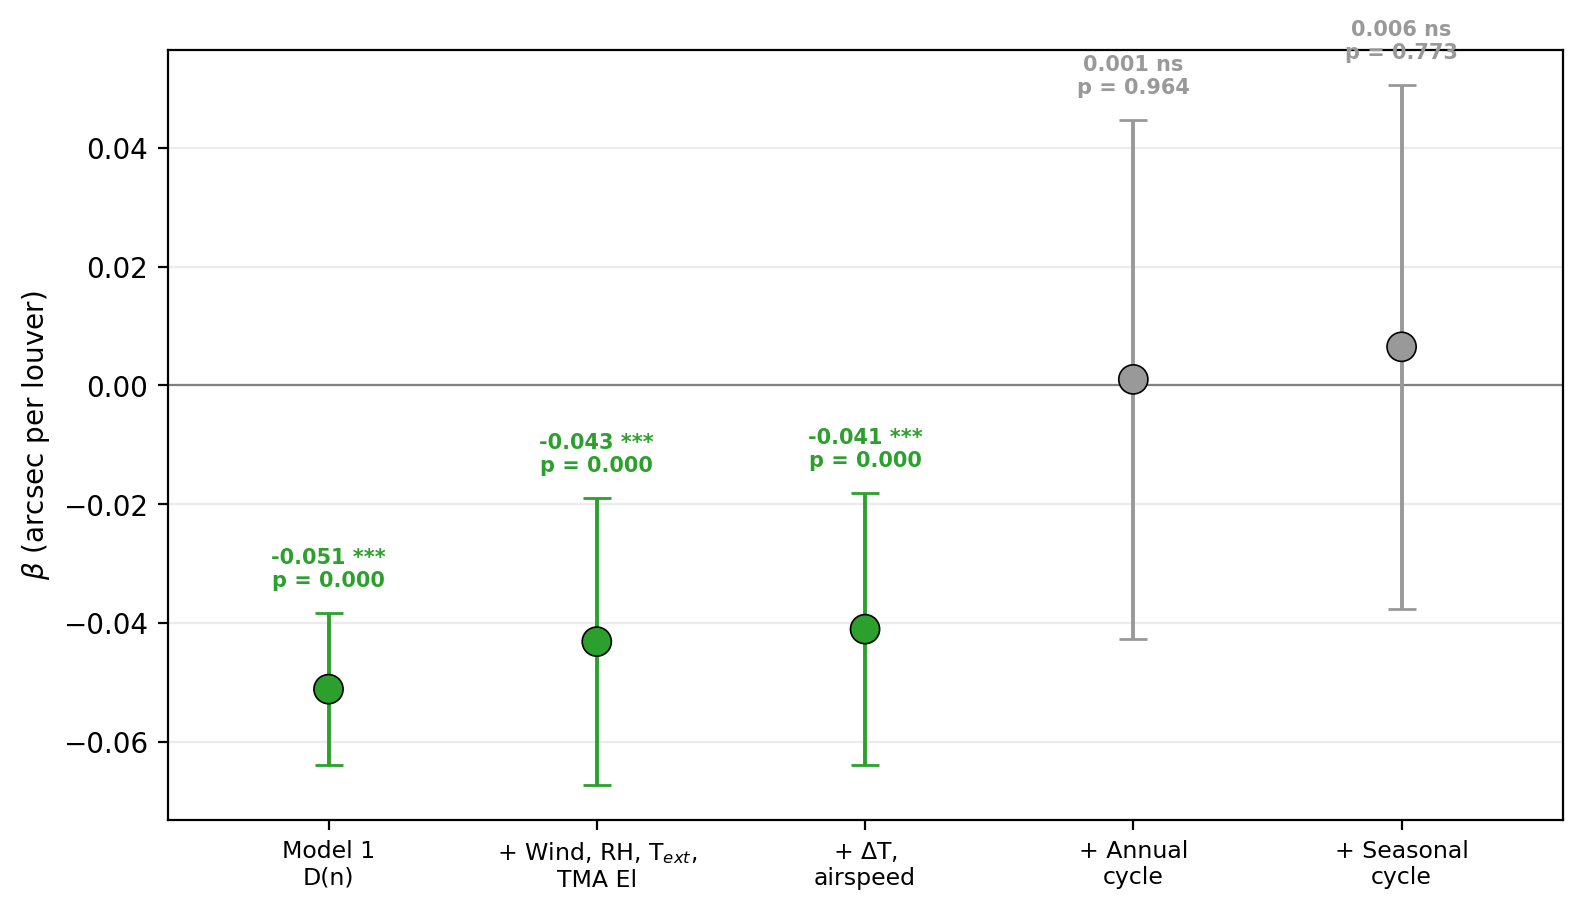
\includegraphics[width=0.98\linewidth]{model1.png}
    \caption{Sensitivity of $\beta$ values by covariates involved in model 1. Green dots shows the physical covariate models. Gray dots include the annual/seasonal cycles in the model. Error bars show 95\% confidence intervals.}
    \label{fig:model1}
\end{figure}

\subsection{Model 2: Within Night Fixed-Effects Regression}
Given that the $\beta$ estimate from model 1 is highly dependent on seasonal cycles another model and data analysis approach needs to be explored. Model 2 is focused on finding within night effects when the louvers changed their configuration while on-sky, we consider negligible the seasonal impact within a given night. It applies an OLS regression of $IQ_{db}$ per exposure on $D(n)$ within the same night. The model can be described as follows:

$IQ_{db}(i) = \alpha_n + \beta \cdot {D(n)}_i + \gamma \cdot {Xcov}_i + \delta \cdot \text{hours sunset}_i + \varepsilon_i $

Where:
\begin{itemize}
	\item $D(n)_{i}$ is the step function that traces the number of operational louvers within a night ($n$) per exposure ($i$).
	\item $\beta$ is the estimation of how much $IQ_{db}$ change per louver.
	\item ${Xcov}_i$ are the covariates considered for each exposure within a given night for this model: external wind speed, external temperature, and TMA elevation.
	\item $\text{hours sunset}_i $ are the hours since sun elevation $\leq -10$ deg per exposure for a given night.
	\item $\varepsilon_i$ are the residual errors per exposure within a given night.
\end{itemize}

Under this model $\beta$ gather the total louver impact in $IQ_{db}$ and $\delta$ gives us the within night $IQ_{db}$ improvement trend since we can be biased in the louver analysis towards having better $IQ_{db}$ once the dome is thermalized within a single night. The covariates included in the within night model are "external" to the louvers within a given night. Model 2 assumes then that the only systematic difference between having the louvers open/close (after controlling for the time of the night and the considered covariates) is the louver configuration. It is worth to note that the time to open/close a louver is not induced by environmental conditions, and the open/close movements are "binary" and not gradual apertures. With this approach, we find a $\beta$ value of $-0.008\pm0.003$ arcsec per louver ($p=0.006$). The model reports a value for $\delta$ of  $-0.023$ arcsec per hour after sunset (p $<$ 0.0001), therefore, within a single night the dome equilibration is the main driver for image quality. If we consider the measured impact in a 8 hours time span, we are accounting about $0.18$ arcsec of image quality improvement. Being this one of the main reasons under our operational stage to streamline daytime activities reaching dome thermal equilibration as soon as possible. If we do not consider the thermal equilibration term the value for $\beta$ increases to $-0.009\pm0.004$ arcsec per louver ($p=0.025$). These result hints to part of the louver effect is driven by the image quality equilibration trend (i.e., image quality improves as the night progresses). 

The results of the within night louver model are shown in Figure \ref{fig:model2}.  The left panel shows the non-modeled louver --$IQ_{db}$ raw relationship separated between the exposures were the louver transition was done between fewer/more louvers (being the zero to six transition the dominant for each box plot respectively). The median $IQ_{db}$ is lower when more louvers are open and its change is found as $\Delta$median\,$=-0.035$ arcsec, given that the typical transition included six louvers the difference translates to $\approx -0.006$ arcsec per louver consistent with the model result of $-0.008\pm0.003$ arcsec per louver. The small difference is expected since the raw values do not control for covariates or hours after sunset. The right panel on Figure \ref{fig:model2} shows the residuals of $IQ_{db}$ vs. the louver count residuals after removing the hours after sunset, and covariates effects from both variables. Since both axes are showing what is left in the model after all the model terms are accounted for, in the case of null impact from the louvers the scatter would be flat. 

The slope of the regression line gives the reported within night model $\beta=-0.008$ arcsec per louver ($p = 0.006$, CI $[-0.013, -0.002]$) showing the louver effect in the model. It is important to note that the vertical scatter is expected since individual $IQ_{db}$ measurements are dominated by factors other than the louvers. The $R^2_{\text{adj}}=0.647$ value on the model regression can be read as the model ability to explain the $\sim$65\% of the exposure $IQ_{db}$ variation, therefore the remaining 35\% unexplained variance includes mainly atmospheric turbulence. Despite the large vertical scatter in individual exposures, the slope ($\beta$) is precisely estimated because the large number of exposures (3694) averages out the noise. The three data clusters along the x-axis reflect the "binary" nature of louver transitions (most of them from 0 to 6 louvers) after night mean removal. Balanced sets in the 0 to 6 louver transition would gather in a night mean value residual of $-3$ (mean number of louvers in a night $\approx 3$, residual $\approx 0 -3 =-3$), balanced sets with 6 to 0 louver transitions would gather in a night residual value of 3, whereas unbalanced nights would have residuals clustered around zero. 
 
As a final sanity check, we also run model 2 dropping each night considered in the dataset. As a result, no single night exceeds the 25\% influence in the reported $\beta$ value. The values found are in the range $[-0.0093, -0.0061]$ arcsec per louver, being all negative and within the uncertainties reported.                                                                                                                                                                                                                                                                                                                                                                                                                                                       

\begin{figure}[!h]
    \centering
    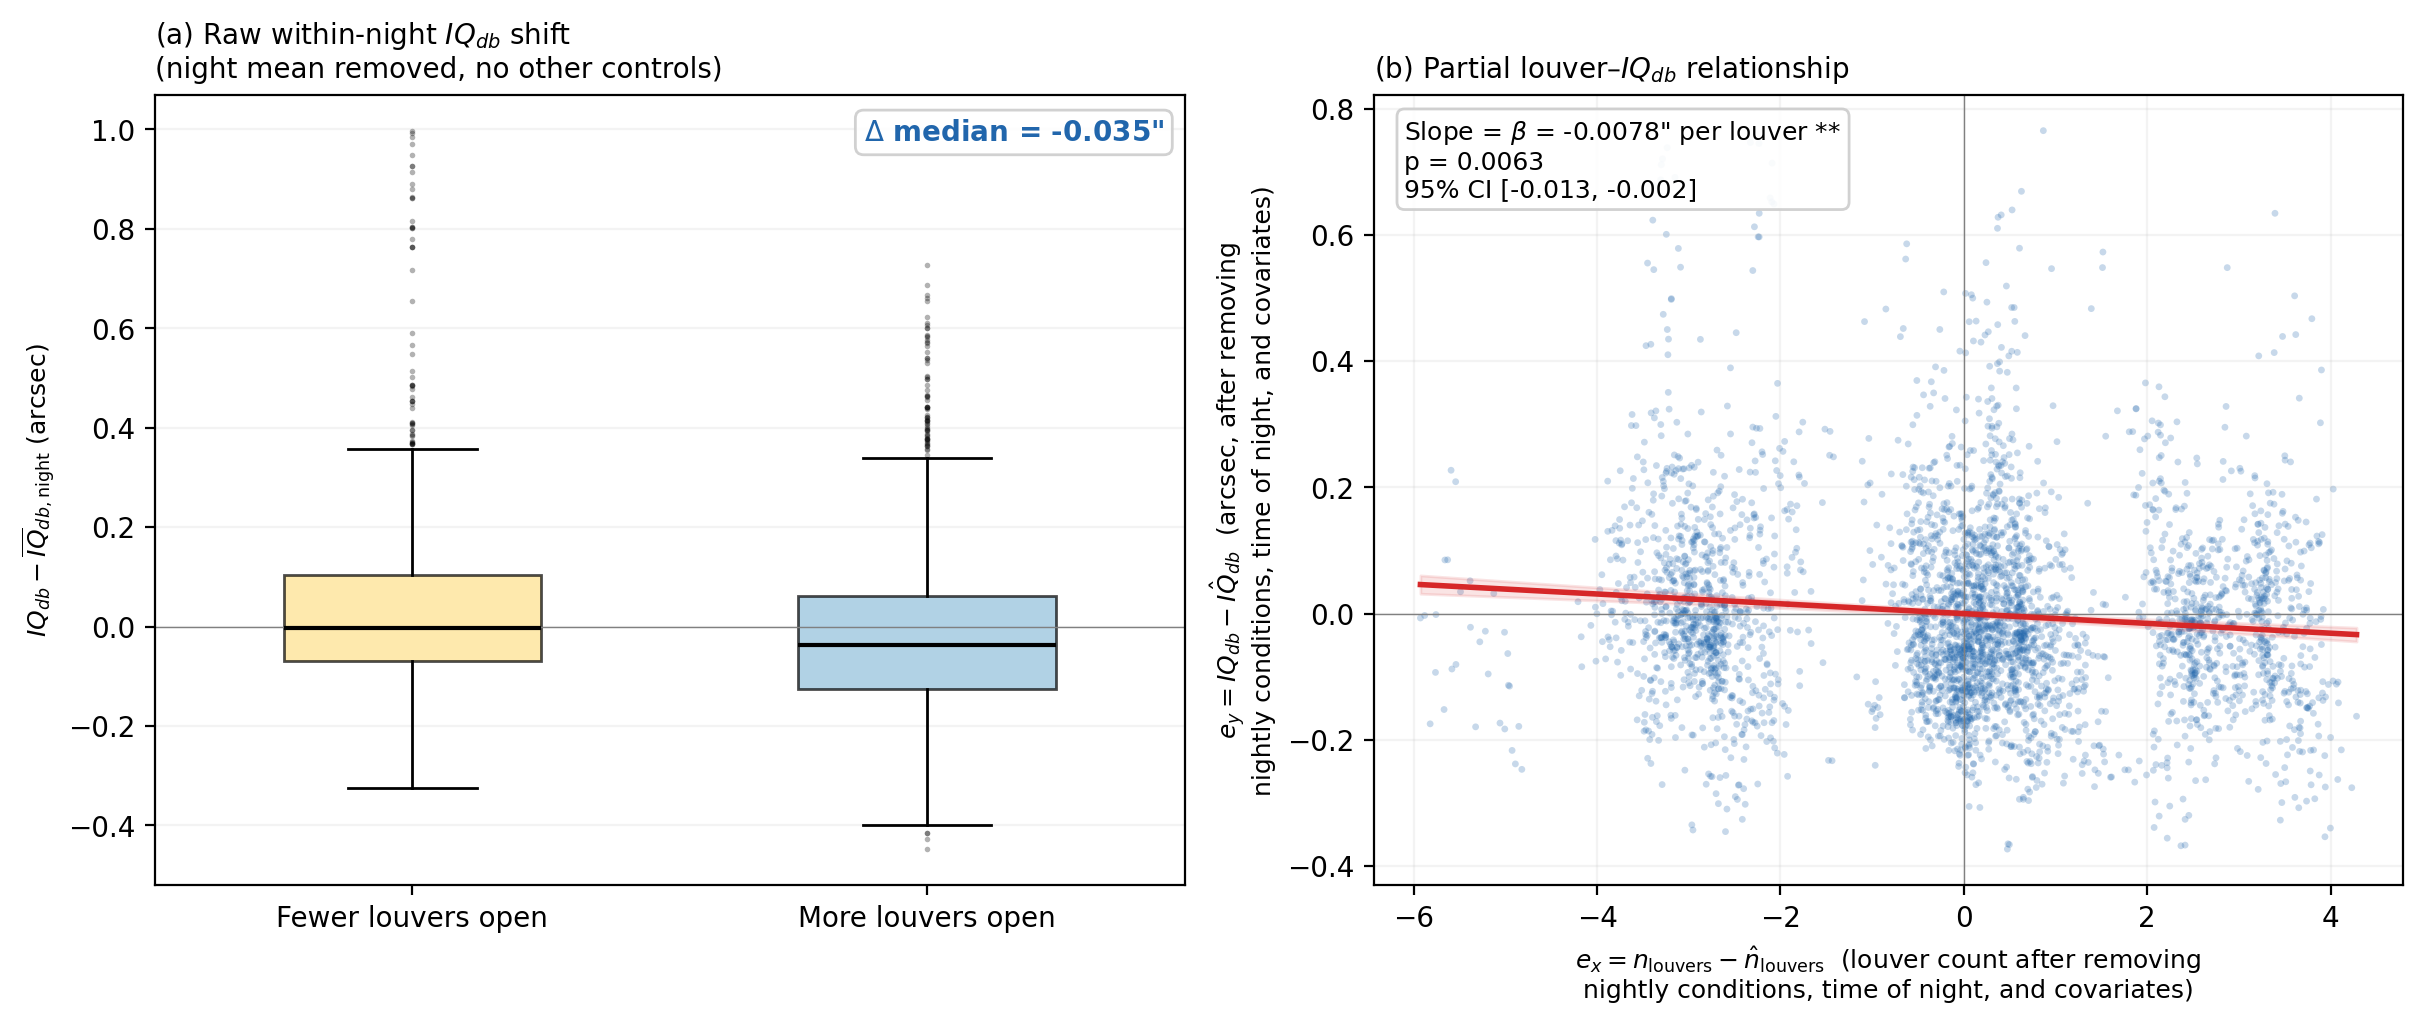
\includegraphics[width=0.98\linewidth]{model2.png}
    \caption{Within Night louver effect on $IQ_{db}$ from 10 switching nights (3694 exposures). (a) Raw change: $IQ_{db}$ relative to the night mean for exposures with fewer vs. more louvers open. (b) Partial regression: residuals of $IQ_{db}$ vs. residuals of louver count after removing hours after sunset, and covariates from both variables. In red the slope of the regression line. Colored band reports the 95\% confidence interval for the slope ($\beta$).}
    \label{fig:model2}
\end{figure}

\section{Conclusions}
The effect of each louver in dome seeing lies between the range $-0.041$ and $-0.008$ arcsec per louver, where the upper limit is highly contaminated by seasonal trends to be refined once we have larger dataset. The lower limit of $-0.008\pm0.003$ arcsec per louver given by the within night regression model is the most robust by the time of writing. It is not related with seasonal trends, it is controlled for the time of the night and the considered covariates. With a total of six louvers we have an improvement of $-0.048$ arcsec on our image quality metric, this increases to $-0.096$ arcsec with twelve louvers and to $-0.272$ arcsec with the envisioned entire system of 34 louvers, assuming a linear extrapolation. If the estimated contribution to delivered image quality by dome seeing is 0.X arcsec. A $-0.272$ arcsec improvement represents $\sim$X\% of the dome seeing budget.

We would like to stress that the louver commissioning coincided with austral seasonal transitions, changes in the number of louvers and even the implementation of pneumatic louvers without telemetry control. For all the venting scenarios discussed in this document we still lack at least one entire year of data. Nevertheless, we do think we are at good position to start the integration of related but spread analysis on dome seeing, as well as to start the refinement on our image quality metric to have an overall vision of dome seeing in the Simonyi telescope.  


\appendix

\section{Acknowledgements}

This material is based upon work supported in part by the National Science Foundation through Cooperative Agreements AST-1258333 and AST-2241526 and Cooperative Support Agreements AST-1202910 and AST-2211468 managed by the Association of Universities for Research in Astronomy (AURA), and the Department of Energy under Contract No.\ DE-AC02-76SF00515 with the SLAC National Accelerator Laboratory managed by Stanford University. Additional Rubin Observatory funding comes from private donations, grants to universities, and in-kind support from LSST-DA Institutional Members.

The statistical analysis pipeline was developed with assistance from Anthropic Claude Opus 4.6. All scientific interpretation and editorial decisions were made by the authors. 

% Include all the relevant bib files.
% https://lsst-texmf.lsst.io/lsstdoc.html#bibliographies
\section{References} \label{sec:bib}
\renewcommand{\refname}{} % Suppress default Bibliography section
\bibliography{local,lsst,lsst-dm,refs_ads,refs,books}

% Make sure lsst-texmf/bin/generateAcronyms.py is in your path
\section{Acronyms} \label{sec:acronyms}
\input{acronyms.tex}
% If you want glossary uncomment below -- comment out the two lines above
%\printglossaries





\end{document}
